\chapter{Methodik}
\label{ch:methodik}

\section{Kodierung}
\label{ch:methodik_kodierung}
\subsection{OvA Kodierung}
Bei der standardmäßig verwendeten One-vs-All Kodierung befindet sich am Ende des Netzes eine \textit{Softmax}-Schicht, die bei $K$ Klassen $K$ Ausgabewerte produziert.

Die Netzausgabe hat die Form $\overrightarrow{\widehat{y}_{OvA}} = \begin{bmatrix}
\widehat{y}_1 & \widehat{y}_2 & ... & \widehat{y}_i & ... & \widehat{y}_{K-1} & \widehat{y}_K
\end{bmatrix} $.\\

Dabei summieren sich alle Werte im Ausgabevektor $\overrightarrow{\widehat{y}_{OvA}}$ zu $1$ auf 
\[1 = \sum_{i=1}^K{\widehat{y}_i} \qquad \text{mit } \widehat{y}_i \in \overrightarrow{\widehat{y}_{OvA}}\]
und bilden somit einen Wahrscheinlichkeitsvektor, bei dem der Wert $\widehat{y}_i$ die Wahrscheinlichkeit angibt, mit der das zu klassifizierende Bild der Klasse $i$ zugewiesen wird.\\

Als Fehlerfunktion wird, wie meistens üblich, die \textit{Cross Entropy Loss} Funktion verwendet. Für den \textit{One-Hot}-kodierten Zielvektor $\overrightarrow{y_{OvA}} = \begin{bmatrix} y_1 & y_2 & ... & y_i & ... & y_{K-i} & y_K \end{bmatrix}$ der Klasse $k$ gilt, dass alle Elemente des Vektors $0$ sind außer dem einem Eintrag $y_k$ an der Stelle $k$, der den Wert $1$ besitzt.


Der Cross Entropy Loss wird dann elementweise für den Zielvektor $\overrightarrow{y_{OvA}}$ und die Netzausgabe $\overrightarrow{\widehat{y}_{OvA}}$ berechnet und aufsummiert:
\[L_{CE} = - \sum_{i=1}^K{y_i * \log{(\widehat{y}_i})} \qquad \text{mit } y_i \in \overrightarrow{y_{OvA}}, \quad \widehat{y}_i \in \overrightarrow{\widehat{y}_{OvA}}\]

Da alle $y_i$ außer einem den Wert $0$ besitzen und somit alle Summanden bis auf einen einzigen $0$ betragen, lässt sich die Summe auflösen zu 
\[L_{CE} = - y_k * \log{(\widehat{y}_k)} = -1 * \log{(\widehat{y}_k)} = - \log{(\widehat{y}_k)}\]
mit $k$ als Klassennummer des Trainingsbeispiels, zu der es tatsächlich gehört.

Da die Logarithmusfunktion zwischen 0 und 1 streng monoton steigt, aber in diesem Intervall einen negativen Wertebereich produziert und sich bei\\ $log(1)=0$ ihr Maximum in dem von der Softmax Funktion produzierten Wertebereich von $[0, 1]$ befindet, wird durch Minimierung der Fehlerfunktion $L_{CE}$ effektiv die Wahrscheinlichkeit $\widehat{y}_k$ für die tatsächliche Klasse $k$ maximiert.


\subsection{OvO Kodierung}
Bei der OvO Klassifikation soll die Netzausgabe für $K$ Klassen folgende Form haben:
\[\overrightarrow{\widehat{y}_{OvO}} = \begin{bmatrix}
\widehat{y}_{1vs2} & \widehat{y}_{1vs3} & ... & \widehat{y}_{1vsK} & \widehat{y}_{2vs3} &... & \widehat{y}_{(K-2)vs K} & \widehat{y}_{(K-1)vsK}
\end{bmatrix} \]
Analog zu dem von Pawara et al. genannten Beispiel (s. \cite{pawaraPaper} Kapitel 2.2) mit $K=5$ Klassen produziert das Netz als Ausgabe einen Vektor mit $\frac{5*(5-1)}{2}=10$ Einträgen:
\[\overrightarrow{\widehat{y}_{OvA}} = \begin{bmatrix}
\widehat{y}_{1vs2} & \widehat{y}_{1vs3} & \widehat{y}_{1vs4} & \widehat{y}_{1vs5} & \widehat{y}_{2vs3} & \widehat{y}_{2vs4} & \widehat{y}_{2vs5} & \widehat{y}_{3vs4} & \widehat{y}_{3vs5} & \widehat{y}_{4vs5}
\end{bmatrix} \]
Dabei steht jeder Eintrag $\widehat{y}_{ivsj}$ in dem Vektor für das Klassifikationsergebnis des One-vs-One Klassifikators, der die Klasse $i$ von Klasse $j$ trennt.\\

Der Zielvektor $\overrightarrow{y_{OvO}}$ besitzt die gleiche Form wie die Netzausgabe und repräsentiert das Klassenlabel in der OvO Kodierung. Für seine Einträge $y_{ivsj}$ gilt:
\begin{figure}[H]
\[
y_{ivsj} = 
\begin{cases}
1 & \text{wenn das Klassifikationsbeispiel zu Klasse } i \text{ gehört}\\
-1 & \text{wenn das Klassifikationsbeispiel zu Klasse } j \text{ gehört}\\
0 & \text{sonst}\\
\end{cases}
\]
\caption{Aufbau der Einträge des Zielvektors.}
\label{gl:OvOZielvektor}
\end{figure}

Da bei dem OvO Klassifikationsschema kein Wahrscheinlichkeitsvektor, in dem sich alle Einträge zu $1$ aufsummieren, als Netzausgabe produziert werden soll, kann die \textit{Softmax}-Schicht nicht verwendet werden. Stattdessen wird die $\tanh$-Aktivierungsfunktion verwendet (s. Abb.\ref{fig:tanh}). Diese erzeugt einen Wertebereich zwischen $-1$ und $1$. Somit fällt jeder Wert in der Netzausgabe $\overrightarrow{\widehat{y}_{OvO}}$ in das Intervall $(-1, 1)$. Dass hier das offene Intervall $(-1, 1)$ produziert wird und nicht das abgeschlossene Intervall $[-1, 1]$ wie vom Zielvektor gefordert (s. Gl. \ref{gl:OvOZielvektor}) hat später bei der Berechnung der Loss-Funktion Vorteile.

\begin{figure}[H]
\begin{adjustbox}{width=.65\textwidth, center}
\includesvg{img/2_tanh}
\end{adjustbox}
\caption{Tanh-Aktivierungsfunktion.}
\label{fig:tanh}
\end{figure}

Da keine One-Hot Kodierung mehr verwendet wird, kann die \textit{Cross-Entropy Loss}-Funktion nicht mehr als Fehlerfunktion verwendet werden. Pawara et al. haben in ihrem Paper \cite{pawaraPaper} eine angepasste \textit{Cross-Entropy}-Funktion entwickelt. Für die Berechnung müssen zuerst die Einträge des Zielvektors $\overrightarrow{y_{OvO}}$ und der Netzausgabe $\overrightarrow{\widehat{y}_{OvO}}$ auf das Intervall $[0, 1]$ skaliert werden:
\begin{figure}[H]
\[y_{ivsj}^{'} = \frac{y_{ivsj} + 1}{2}\]
\[\widehat{y}_{ivsj}^{'} = \frac{\widehat{y}_{ivsj} + 1}{2}\]
\caption{Skalierung der Einträge in dem Zielvektor und der Netzausgabe (\cite{pawaraPaper} Kapitel 2.2 Gleichung 5).}
\label{gl:pawaraSkalierung}
\end{figure}

Anschließend wird gemäß der Formel von Pawara et al. der Loss-Wert ausgerechnet (s. Gl. \ref{gl:pawaraLoss}).

\begin{figure}[H]
\[L_{OvO} = - \frac{1}{L} \sum_{l=1}^{L}((y_{l}^{'} * \log{(\widehat{y}_{l}^{'})}) + (1 - y_{l}^{'}) * \log{(1-\widehat{y}_{l}^{'})})\]
mit\\
$\boldsymbol{K}:$ Anzahl an Klassen\\

$\boldsymbol{L}=\frac{K*(K-1)}{2}:$ Länge der Netzausgabe bzw. des Zielvektors\\

$\boldsymbol{y_{l}^{'}}:$ auf $[0, 1]$ skalierter Eintrag des Zielvektors $\overrightarrow{y_{OvO}}$ an $l$-ter Stelle\\

$\boldsymbol{\widehat{y}_{l}^{'}}:$ auf $[0, 1]$ skalierter Eintrag des Netzausgabe-Vektors $\overrightarrow{\widehat{y}_{OvO}}$ an $l$-ter Stelle\\


\caption{Formel zur Berechnung der von Pawara et al. vorgestellten Loss-Funktion (\cite{pawaraPaper} Kapitel 2.2 Gleichung 6).}
\label{gl:pawaraLoss}
\end{figure}

Es wird also für jeden Eintrag $\widehat{y}_{l}^{'}$ in dem Netzausgabe-Vektor mit Hilfe des zugehörigen Eintrages $y_{l}^{'}$ im Zielvektor ein Loss-Wert berechnet und über alle $L$ Einträge in den Vektoren gemittelt. Der Wertebereich der Einträge beider Vektoren liegt wegen der Skalierung (s. Gl. \ref{gl:pawaraSkalierung}) im Intervall $[0,1]$. Da dies jedoch zu numerischen Problemen führt, da z.B. $\log{(0)}$ nicht definiert ist, muss der Wertebereich auf $(0, 1)$ bzw. näherungsweise auf $[0.00001, 0.99999]$ beschränkt werden (vgl. \cite{pawaraPaper} Kapitel 2.2).
In dem auf $[0, 1]$ skalierten Zielvektor sind daher abgesehen von der näherungsweisen Beschränkung des Wertebereichs Einträge mit folgenden Werten möglich:
\[
y_{ivsj}^{'}=
\begin{cases}
1 & \text{wenn das Klassifikationsbeispiel zu Klasse } i \text{ gehört}\\
0 & \text{wenn das Klassifikationsbeispiel zu Klasse } j \text{ gehört}\\
0.5 & \text{sonst}\\
\end{cases}
\]

Für $y_{l}^{'} = 1$ reduziert sich ein Summand der Summe aus Gl. \ref{gl:pawaraLoss} zu
\[-((\boldsymbol{1} * \log{(\widehat{y}_{l}^{'})}) + (1 - \boldsymbol{1}) * \log{(1-\widehat{y}_{l}^{'})}) = -\log{(\widehat{y}_{l}^{'})}\]

Für $y_{l}^{'} = 0$ reduziert sich ein Summand der Summe aus Gl. \ref{gl:pawaraLoss} zu
\[-((\boldsymbol{0} * \log{(\widehat{y}_{l}^{'})}) + (1 - \boldsymbol{0}) * \log{(1-\widehat{y}_{l}^{'})}) = -\log{(1-\widehat{y}_{l}^{'})}\]

Für $y_{l}^{'} = 0.5$ reduziert sich ein Summand der Summe aus Gl. \ref{gl:pawaraLoss} zu
\[-((\boldsymbol{0.5} * \log{(\widehat{y}_{l}^{'})}) + (1 - \boldsymbol{0.5}) * \log{(1-\widehat{y}_{l}^{'})}) = - (0.5 * \log{(\widehat{y}_{l}^{'})} + 0.5 * \log{(1-\widehat{y}_{l}^{'})})\]

\todo{Plots für die 3 Fälle einfügen (Dont Care's fließen mit ein!)}
\todo{Umsetzung: OvO Matrix, Klassifizierung}
\todo{Warum Datensätze mit 3 Klassen verwendet wurden}

\subsection{Alternative Kodierungsmethoden}
\todo{alternative Kodierungsmöglichkeiten beschreiben (s. Paper, z.B. Error correcting codes)}

\newpage
\section{Datensätze}
\label{ch:methodik_datensaetze}
Für die Experimente wurden 5 verschiedene Datensätze verwendet: Agrilplant \cite{pawaraWebsiteDatensaetze}, Cifar \cite{cifar10}, Monkey \cite{pawaraWebsiteDatensaetze}, SwedishLeaves \cite{swedishLeaves} und Tropic \cite{pawaraWebsiteDatensaetze}.

Für jeden Datensatz existieren Exemplare mit verschiedenen Anzahlen an Klassen (s. Abb. \ref{fig:DatensatzKlassen}), die zukünftig jeweils mit $<$Datensatzname$><$Klassenanzahl$>$ wie z.B. Agrilplant10 bezeichnet werden.
Die Datensätze mit geringerer Klassenanzahl sind Teilmengen des gesamten Datensatzes, bei denen nur die ersten $k$ Klassen verwendet werden.

Bei allen Datensätzen außer SwedishLeaves (s. Kapitel \ref{ch:methodik_SwedishLeaves}) wird eine 5-Fold Cross Validation angewendet, es werden also 5 Aufteilungen in Train- und Testdaten im Verhältnis 80:20 erstellt, sodass sich jedes Bild genau in einem Fold im Testsplit und in 4 Folds im Trainsplit befindet.

Für die Datensätze Tropic10 und Monkey10 stehen auf der Homepage der Autorin \cite{pawaraWebsiteDatensaetze} die von ihr verwendeten Einteilungen in 5 Folds zur Verfügung. Diese Datensätze, die mit der exakt gleichen Einteilung in 5 Folds verwendet wurden, werden im weiteren Verlauf dieser Arbeit mit dem Präfix\\ \enquote{Pawara-} kenntlich gemacht. Da die gleiche Einteilung in 5 Folds verwendet wurde wie im Paper von Pawara et al. \cite{pawaraPaper} ist die Vergleichbarkeit der reproduzierten Ergebnisse höher.

Für alle anderen Datensätze musste die Einteilung in 5 bzw. für SwedishLeaves 3 Folds neu erstellt werden.
Außerdem wurde für Tropic10 ebenfalls eine eigene 5-Fold Cross Validation erstellt, da die von der Autorin zur Verfügung gestellte Einteilung (s. \cite{pawaraWebsiteDatensaetze}) fehlerhaft ist. Ihre sogenannte 5-Fold Cross Validation besteht bei Tropic10 vermutlich aus fünfmaligem, zufälligem Ziehen eines Verhältnisses 70:30 für Trainings und Testdaten. Dies führt dazu, dass ein eventuell schwierig zu klassifizierendes Bild in mehr als einem Fold im Testsplit vorkommen und somit das Ergebnis abhängig vom Zufall beeinflussen kann.
\todo{In Scatterplots schauen, inwiefern diese Aussage stimmt}

\begin{figure}[H]
\begin{tabular}{|c|c|c|c|c|c|}
\hline 
Anzahl an Klassen & 3 & 5 & 10 & 15 & 20 \\ 
\hline 
Agrilplant & X & X & X &  &  \\ 
Cifar &  &  & X &  &  \\ 
Monkey &  &  & X &  &  \\ 
SwedishLeaves & X & X & X & X &  \\ 
Tropic & X & X & X & & X \\ 
\hline 
\end{tabular} 
\caption{Zum Training verwendete Anzahl an Klassen je Datensatz}
\label{fig:DatensatzKlassen}
\end{figure}

\subsection{Agrilplant}
Der Agrilplant Datensatz \cite{pawaraWebsiteDatensaetze} besteht aus Bildern von Blüten, Früchten und Blättern von Agrarpflanzen.
Es existieren 10 verschiedene Klassen: Apfel, Banane, Traube, Jackfruit, Orange, Papaya, Kaki, Ananas, Sonnenblume und Tulpe (vgl. \cite{pawaraWebsiteDatensaetze}).
\begin{figure}[H]
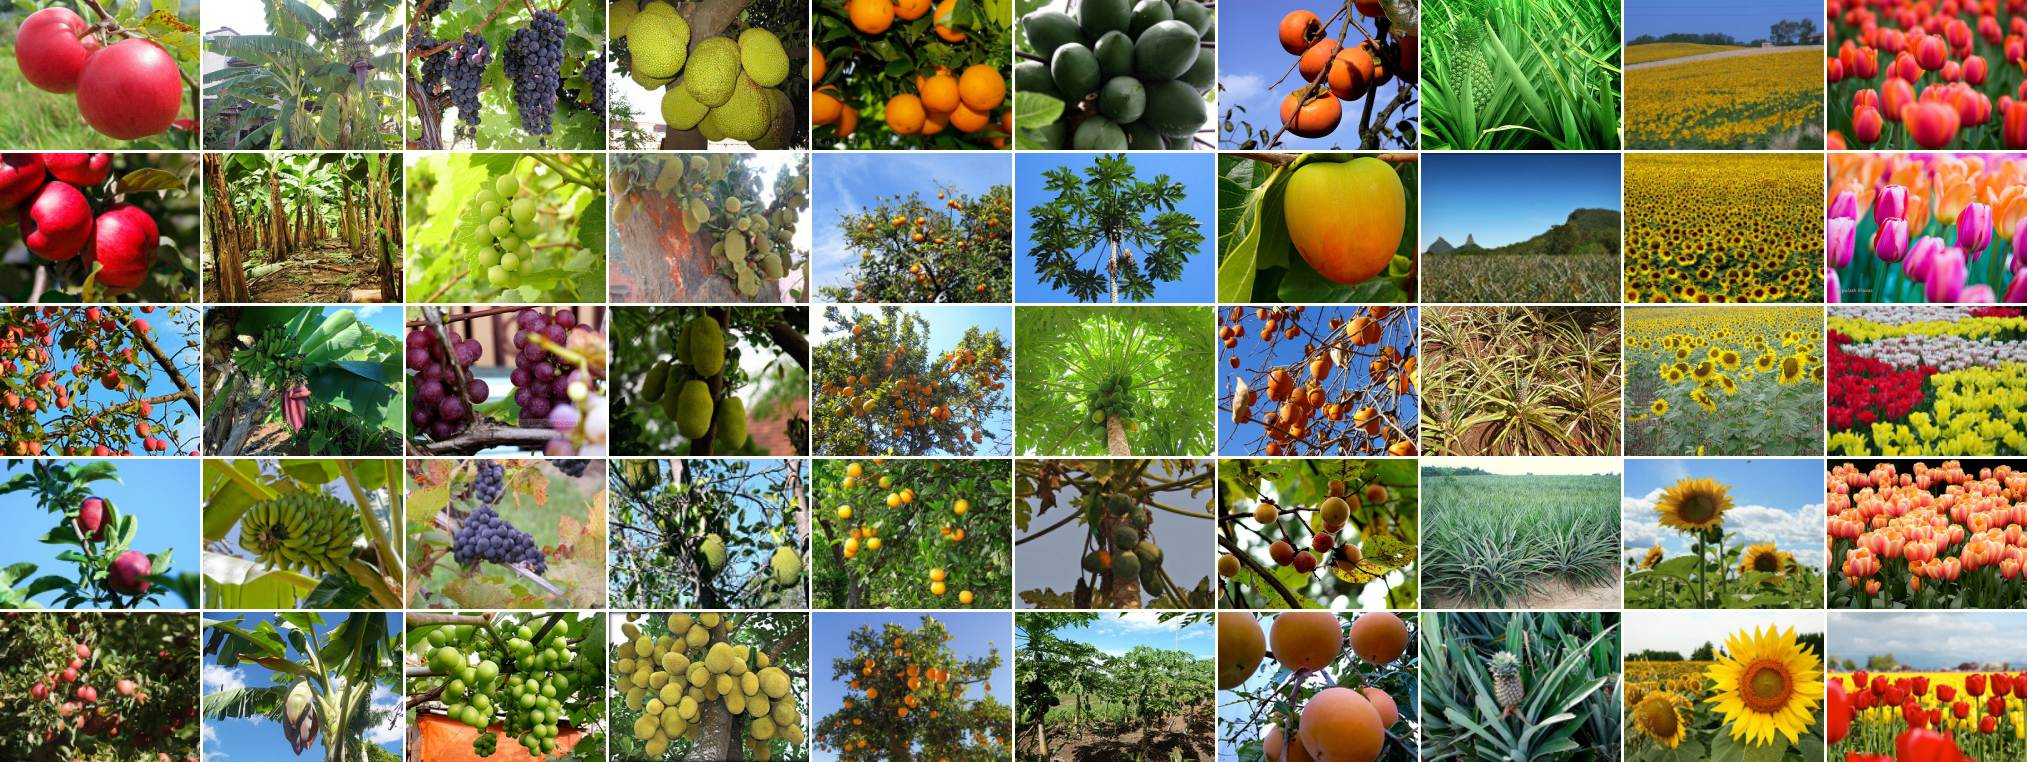
\includegraphics[scale=0.2]{img/2_agrilplant-image.jpg}
\caption{Überblick über die verschiedenen Klassen des Agrilplant Datensatzes \cite{pawaraAgrilplant}.}
\label{fig:agrilplantUeberblick}
\end{figure}

Zum Training wurden zusätzlich zu Agrilplant10 noch zwei weitere Teilmengen des Datensatzes, Agrilplant5 und Agrilplant3, verwendet.

Der Datensatz Agrilplant10 besteht aus 300 Bildern mit einer Auflösung von ca. 200-500 Pixeln je Klasse, also insgesamt 3000 Bilder, und ist damit perfekt ausbalanciert (s. Abb. \ref{fig:Agrilplant10Zusammensetzung}).\\


\begin{figure}[H]
\begin{adjustbox}{width=1.4\textwidth, center}
\includesvg{img/2_agrilplant10_Zusammensetzung}
\end{adjustbox}
\caption{Aufteilung des Agrilplant10 Datensatzes \cite{pawaraWebsiteDatensaetze} in Train- und Testsplits je Fold.}
\label{fig:Agrilplant10Zusammensetzung}
\end{figure}


\subsection{Cifar}
Der Cifar10 Datensatz beinhaltet insgesamt 60.000 Bilder in einer sehr kleinen Auflösung von 32x32 Pixeln. Es existieren 10 Klassen: Flugzeug, Automobil, Vogel, Katze, Hirsch, Hund, Frosch, Pferd, Schiff, Lastkraftwagen (vgl. \cite{cifar10}).
Die Aufteilung in Klassen ist perfekt ausbalanciert mit genau 6.000 Bildern pro Klasse (s. Abb. \ref{fig:Cifar10Zusammensetzung}).
Da die zum Training verwendeten Netze für Bilder in einer Auflösung von 224 bzw. 299 Pixeln ausgelegt sind (vgl. \ref{ch:methodik_netze}) müssen die Bilder von diesem Datensatz ungefähr 8-fach vergrößert werden.\\

Durch die große Anzahl an Bildern und die starke Hochskalierung benötigt das Training viel Zeit und Ressourcen, weshalb Cifar10 nur bei Resnet Scratch verwendet wird.
\todo{Verlinkung setzen auf Trainingsdauer, Aussage wie viel länger als z.B. Tropic20}

Dieser Datensatz wurde zusätzlich zu den anderen ausgewählt um die Aussagekraft der Ergebnisse zu erhöhen, da sich die anderen Datensätze lediglich auf Pflanzen und Affen beschränken. Im wissenschaftlichen Paper von Pawara et al. \cite{pawaraPaper} wird dieser Datensatz nicht behandelt.

\begin{figure}[H]
\begin{adjustbox}{width=1.4\textwidth, center}
\includesvg{img/2_cifar10_Zusammensetzung}
\end{adjustbox}
\caption{Aufteilung des Cifar10 Datensatzes \cite{cifar10} in Train- und Testsplits je Fold.}
\label{fig:Cifar10Zusammensetzung}
\end{figure}


\subsection{Monkey}
Für den Monkey Datensatz existieren 2 Versionen: Pawara-Monkey10 und Pawara-uMonkey10 mit absichtlich nicht ausbalancierten Anzahlen an Bildern je Klasse, um zu untersuchen wie die beiden Klassifikationsschemata auf schlecht ausbalancierten Datensätzen abschneiden (vgl. \cite{pawaraWebsiteDatensaetze}). Beide Versionen bestehen aus Bildern aus 10 Klassen von verschiedenen Affenarten aufgenommen in freier Wildbahn aus unterschiedlichen Perspektiven (s. Abb. \ref{fig:monkey10Ueberblick}) und wurden in genau der gleichen Aufteilung in Folds bei den Experimenten im Paper von Pawara et al. \cite{pawaraPaper} verwendet.
Die Bilder haben eine Auflösung von ca. 180 bis zu 6.000 Pixeln.
\begin{figure}[H]
\centering
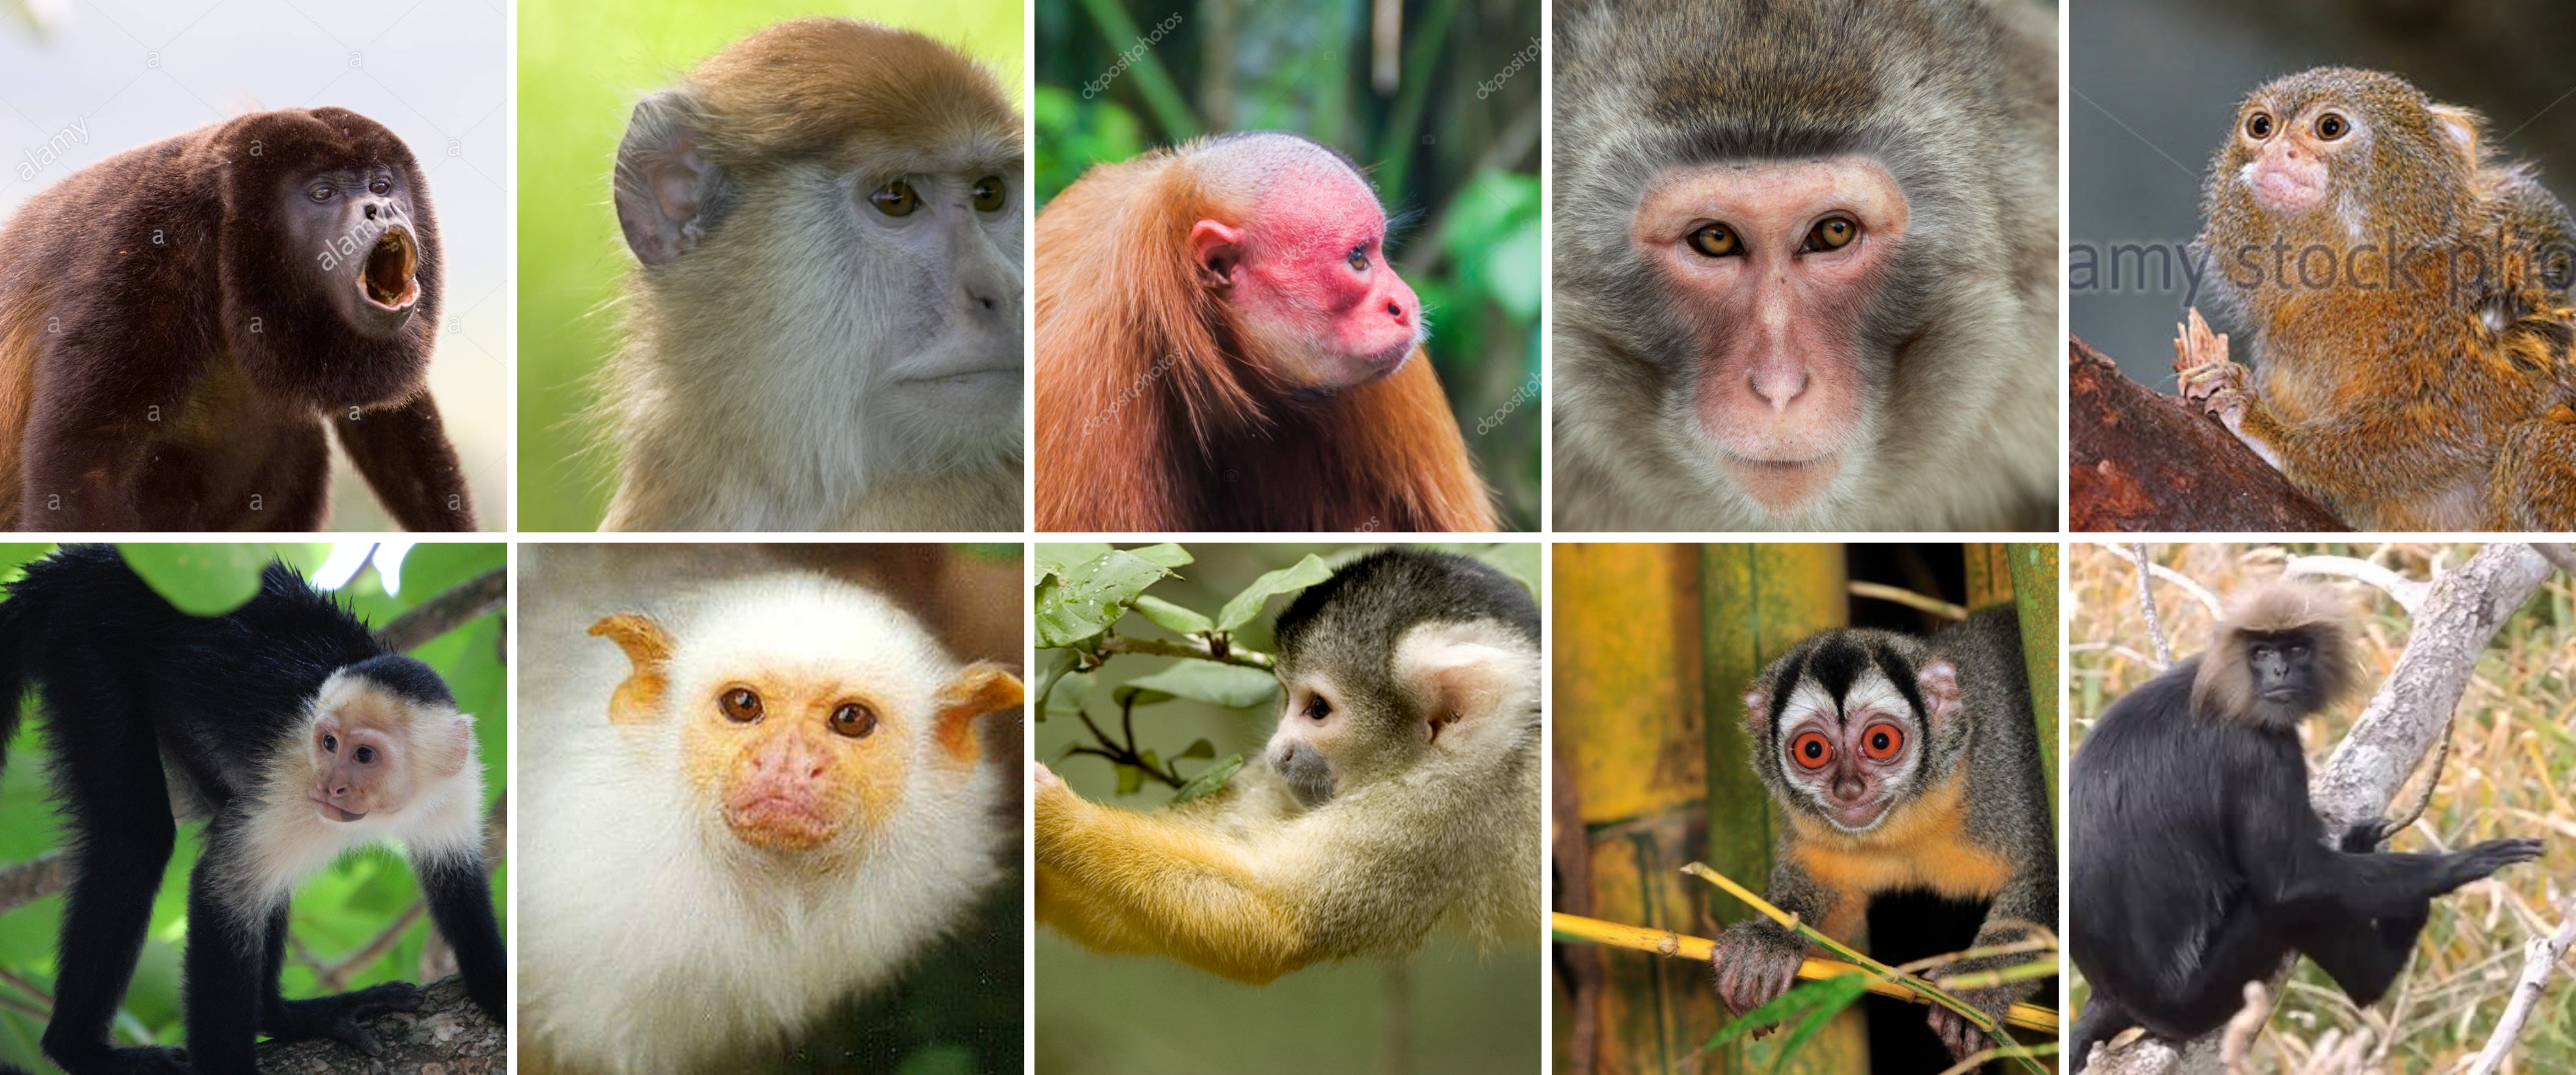
\includegraphics[scale=0.08]{img/2_monkey10-image.jpg}
\caption{Überblick über die verschiedenen Klassen des Monkey10 Datensatzes \cite{pawaraMonkey}.}
\label{fig:monkeyUeberblick}
\end{figure}

Der Pawara-Monkey10 Datensatz besteht aus insgesamt 1370 Bildern und ist mit 131 bis 152 Bildern je Klasse noch relativ gut ausbalanciert (s. Abb \ref{fig:Pawara-Monkey10Zusammensetzung}).\\

Im Gegensatz dazu ist der Datensatz Pawara-uMonkey10 weder in der Anzahl an Bildern pro Klasse noch in der Größe der Folds im Trainsplit ausbalanciert (s. Abb. \ref{fig:Pawara-uMonkey10Zusammensetzung}). 


\begin{figure}[H]
\begin{adjustbox}{width=1.4\textwidth, center}
\includesvg{img/2_pawara-monkey10_Zusammensetzung}
\end{adjustbox}
\caption{Aufteilung des Pawara-Monkey10 Datensatzes \cite{pawaraWebsiteDatensaetze} in Train- und Testsplits je Fold.}
\label{fig:Pawara-Monkey10Zusammensetzung}
\end{figure}
\begin{figure}[H]
\begin{adjustbox}{width=1.4\textwidth, center}
\includesvg{img/2_pawara-umonkey10_Zusammensetzung}
\end{adjustbox}
\caption{Aufteilung des unbalancierten Pawara-uMonkey10 Datensatzes \cite{pawaraWebsiteDatensaetze} in Train- und Testsplits je Fold.}
\label{fig:Pawara-uMonkey10Zusammensetzung}
\end{figure}





\subsection{SwedishLeaves}
\label{ch:methodik_SwedishLeaves}
Der SwedishLeaves Datensatz besteht aus Bildern von Blättern schwedischer Bäume, die zentriert auf einem weißen Hintergrund liegen (s. Abb. \ref{fig:swedishLeavesUeberblick}). Dadurch besitzen Bilder innerhalb einer Klasse eine hohe Ähnlichkeit.

\begin{figure}[H]
\centering
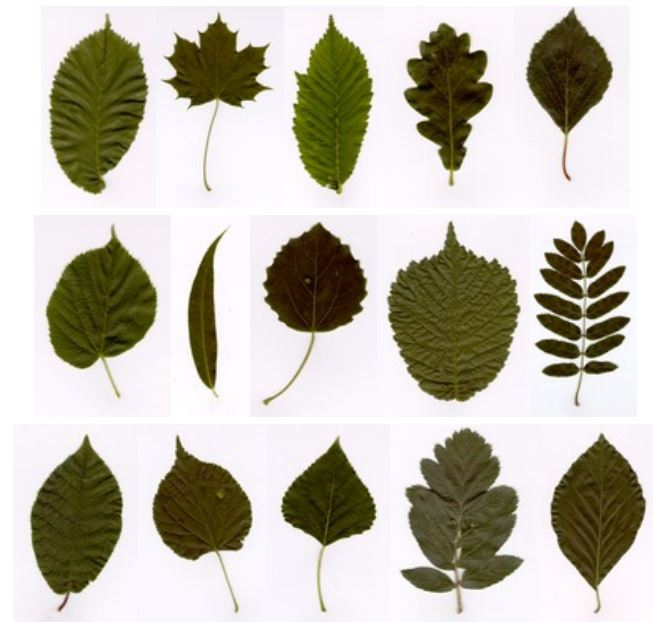
\includegraphics[scale=0.8]{img/2_swedishLeaves-image.jpg}
\caption{Überblick über die verschiedenen Klassen des SwedishLeaf Datensatzes \cite{pawaraMonkey}.}
\label{fig:swedishLeavesUeberblick}
\end{figure}

In den Experimenten von Pawara et al. \cite{pawaraPaper} wurde fünfmal ein Verhältnis von 1:2 für Trainings- und Testdaten aus den 75 Bildern pro Klasse gezogen (vgl. \cite{pawaraPaper} Kapitel 3.1.3), sodass im Testsplit doppelt so viele Bilder sind wie im Trainsplit.

Da hierbei offensichtlich Doppelungen zwischen den Folds entstehen und die verwendete Einteilung der Autorin des Papers \cite{pawaraPaper} nicht verfügbar ist, habe ich mich dafür entschieden die 75 Bilder pro Klasse in 3 Gruppen zu je 25 Bildern auf zu teilen und daraus 3 Folds mit einem Verhältnis von 1:2 für Trainings und Testdaten zu mischen. Dabei gelangt jedes Bild genau in einem Fold in den Trainsplit und in zwei Folds in den Testsplit. Es entsteht quasi eine 3-Fold Cross Validation mit vertauschtem Train- und Testsplit (s. Abb. \ref{fig:swedishLeavesZusammensetzung}).

Zusätzlich zu SwedishLeaves15 wurde mit drei weiteren Teilmengen des Datensatzes gearbeitet: SwedishLeaves10, SwedishLeaves5 und SwedishLeaves3.

\begin{figure}[H]
\begin{adjustbox}{width=1.4\textwidth, center}
\includesvg{img/2_swedishLeaves15_Zusammensetzung}
\end{adjustbox}
\caption{Aufteilung des SwedishLeaves15 Datensatzes \cite{swedishLeaves} in Train- und Testsplits je Fold.}
\label{fig:swedishLeavesZusammensetzung}
\end{figure}

\subsection{Tropic}
In dem Tropic Datensatz \cite{pawaraWebsiteDatensaetze} befinden sich 20 Klassen mit Bildern tropischer Pflanzen und deren Blättern, Blüten und Früchten (s. Abb. \ref{fig:tropicUeberblick}). Da unterschiedliche Teile der Pflanzen aus verschiedenen Blickwinkeln vor vielfältigen Hintergründen wie z.B. Erde, Himmel, Straßen oder Häusern fotografiert wurden ist die Klassifikation im Vergleich zum SwedishLeaves Datensatz \cite{swedishLeaves} (s. Kapitel \ref{ch:methodik_SwedishLeaves}) wesentlich anspruchsvoller.


\begin{figure}[H]
\centering
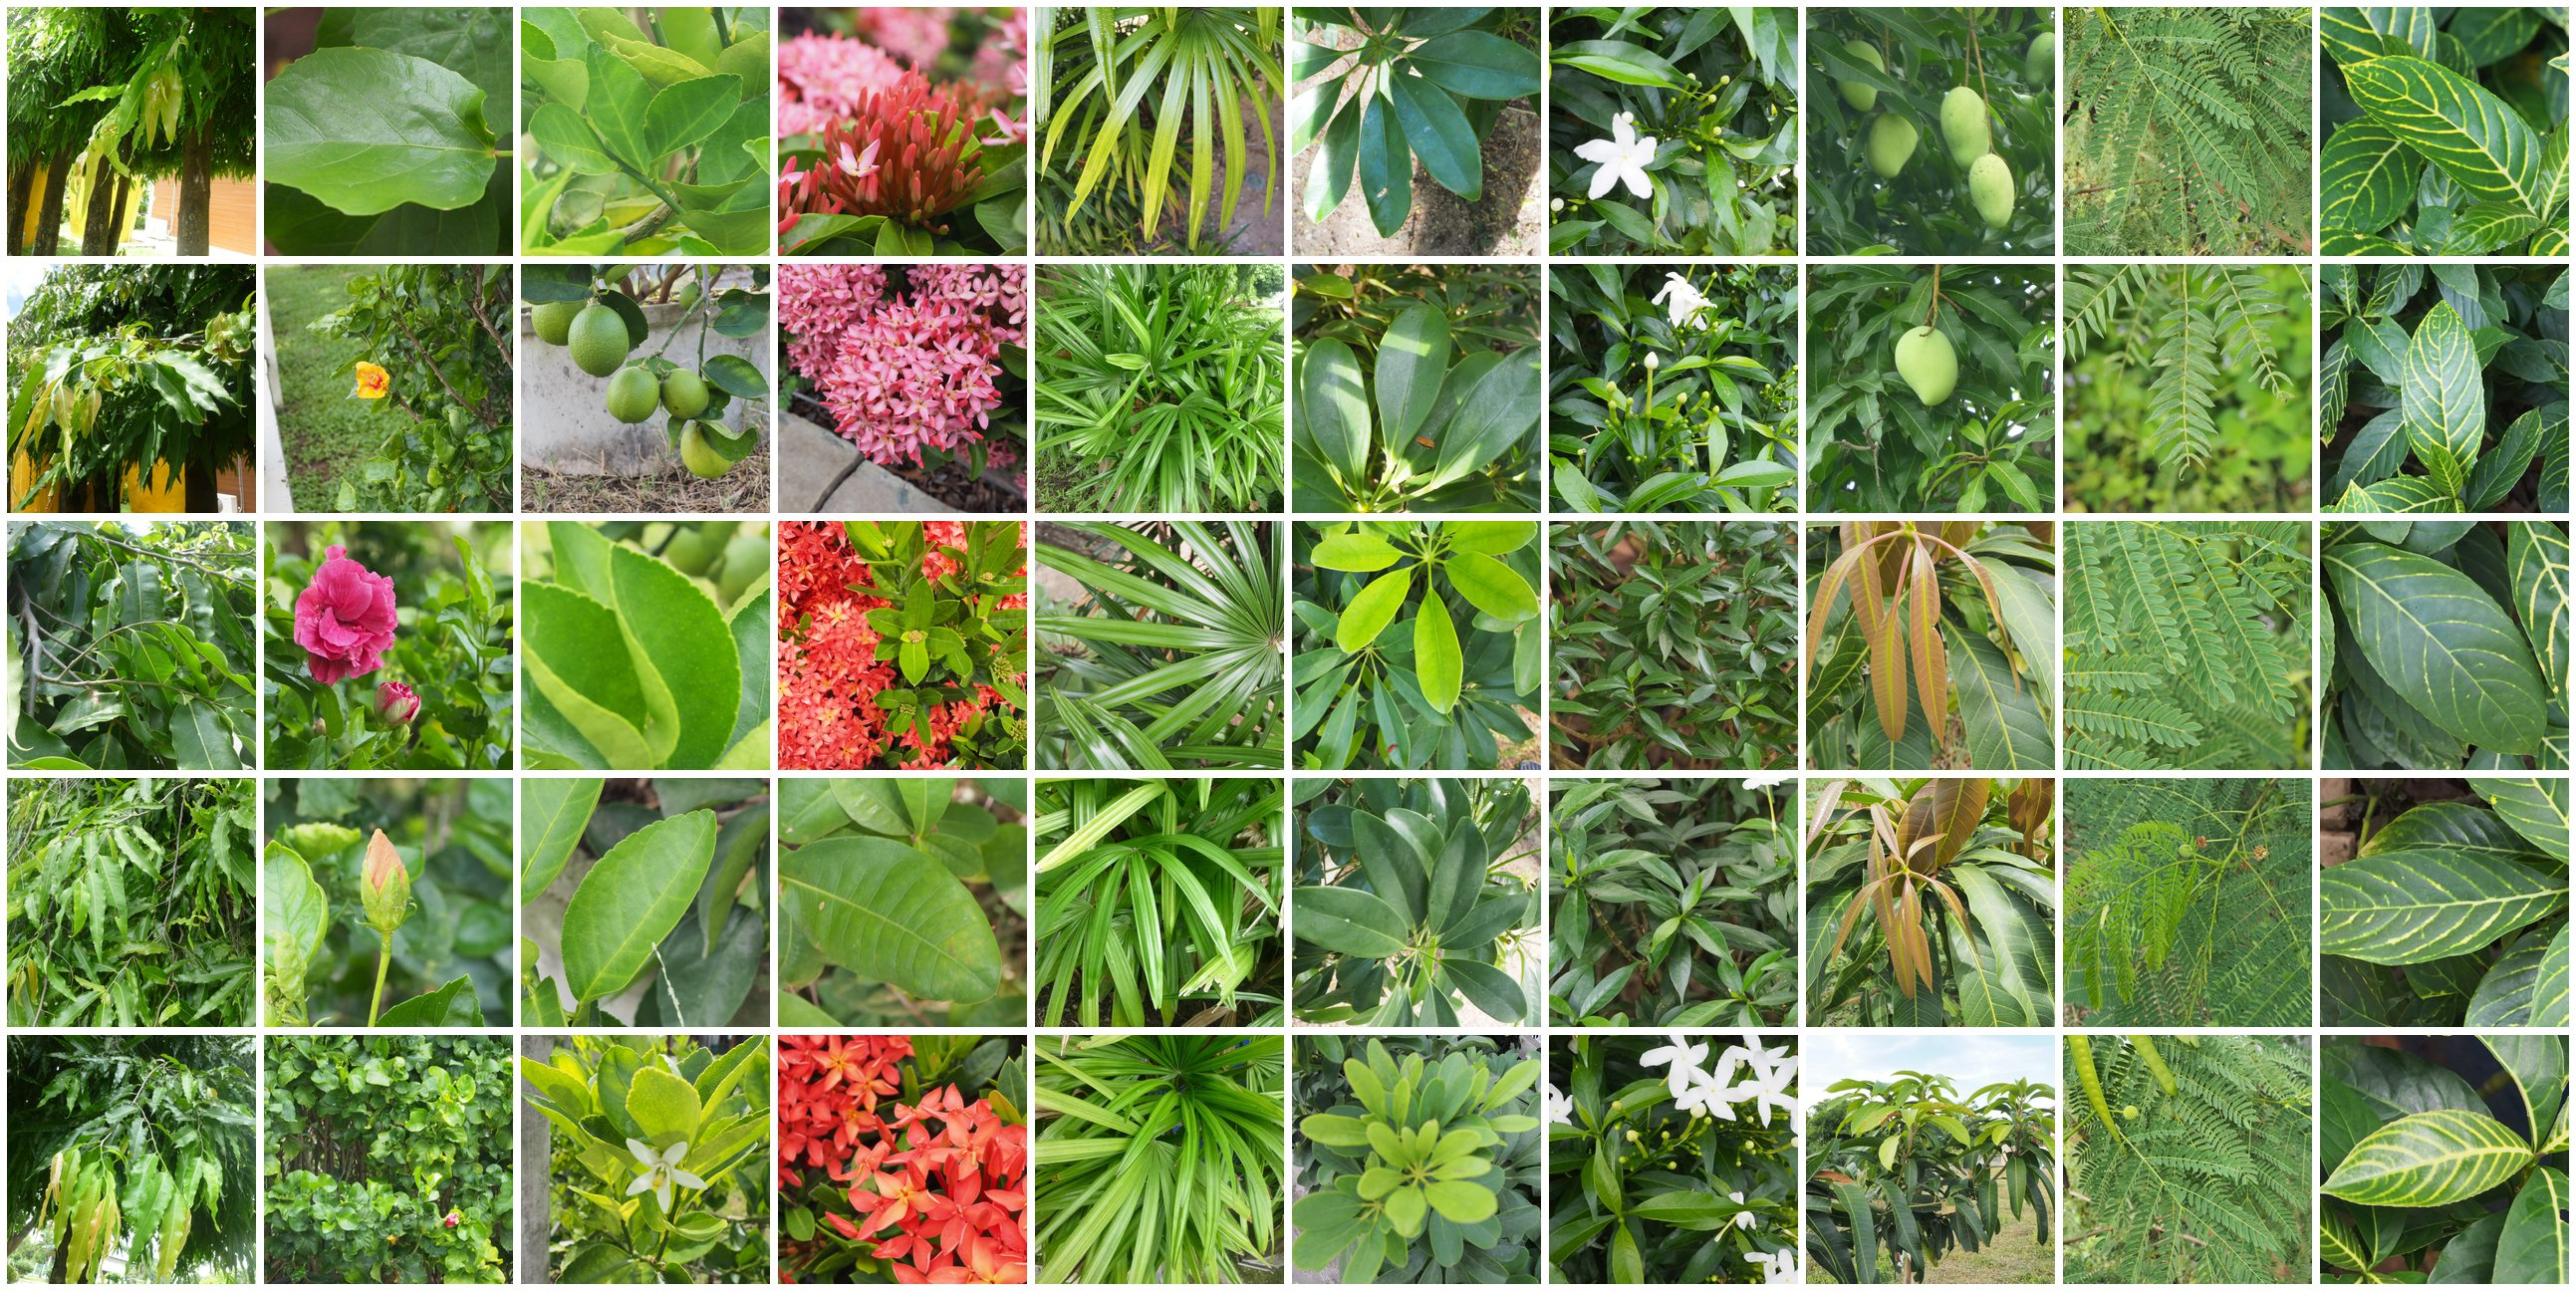
\includegraphics[scale=0.14]{img/2_tropic10-image.jpg}
\caption{Überblick über die verschiedenen Klassen des\\
Tropic Datensatzes \cite{pawaraTropic}.}
\label{fig:tropicUeberblick}
\end{figure}

Pro Klasse existieren 221-371 Bilder (s. Abb. \ref{fig:tropic20Zusammensetzung} und Abb. \ref{fig:pawaraTropic10Zusammensetzung}) in einer Auflösung von 250x250 Pixeln.

Es wurden Teilmengen von diesem Datensatz mit 20, 10, 5 und 3 Klassen zum Vergleich der beiden Klassifikationsschemata verwendet. Außerdem wurde die von Pawara et al. im Paper \cite{pawaraPaper} verwendete Einteilung in Folds \textit{Pawara-Tropic10} \cite{pawaraWebsiteDatensaetze} benutzt, bei der die 5-Fold Cross Validation aus fünfmaligem, zufälligem Ziehen eines Verhältnisses 70:30 für Trainings- und Testdaten besteht (s. Abb. \ref{fig:pawaraTropic10Zusammensetzung}).
Zusätzlich existiert noch ein Tropic52 Datensatz \cite{pawaraWebsiteDatensaetze} mit 52 Klassen, der aber weder im Paper von Pawara et al. \cite{pawaraPaper} noch in dieser Bachelorarbeit behandelt wird.

\begin{figure}[H]
\begin{adjustbox}{width=1.4\textwidth, center}
\includesvg{img/2_tropic20_Zusammensetzung}
\end{adjustbox}
\caption{Aufteilung des Tropic20 Datensatzes \cite{pawaraWebsiteDatensaetze} in Train- und Testsplits je Fold.}
\label{fig:tropic20Zusammensetzung}
\end{figure}
\begin{figure}[H]
\begin{adjustbox}{width=1.4\textwidth, center}
\includesvg{img/2_pawara-tropic10_Zusammensetzung}
\end{adjustbox}
\caption{Aufteilung des Pawara-Tropic10 Datensatzes \cite{pawaraWebsiteDatensaetze} in Train- und Testsplits je Fold.}
\label{fig:pawaraTropic10Zusammensetzung}
\end{figure}


\section{Trainingsparameter}
\label{ch:methodik_parameter}
Um zu untersuchen wie OvO und OvA im Vergleich zueinander in verschiedenen Situationen abschneiden, werden die folgenden Trainingsparameter für beide Klassifikationsschemata variiert.
Dadurch kann eine allgemeinere Aussage über die Vor- und Nachteile der OvO und OvA Klassifikation getroffen werden, da man durch die Variation der Trainingsparameter einen größeren Bereich an potentiellen Anwendungsfällen abdeckt.

Außerdem kann durch die verschiedenen Trainingsparameter analysiert werden, in welchen Situationen die OvO Klassifikation seine theoretischen Vorteile in der Praxis besonders gut ausnutzen kann und wann sich eine Implementation des OvO Klassifikationsschemas eher nicht lohnt.


\begin{figure}[H]
\begin{tabular}{|c|c|c|}
\hline 
\multirow{2}{*}{\textbf{Parameter}} & \multirow{2}{*}{\textbf{mögliche Werte}} & \textbf{Anzahl} \\ 
& & \textbf{möglicher Werte} \\
\hline 
Framework & \{TF1.13.1, TF2.4.1, torch\} & 3\\
\hline
Datensatz & s. Kapitel \ref{ch:methodik_datensaetze} & 15\\
\hline 
\multirow{2}{*}{Netztyp} & \{ResNet-50, InceptionV3, & \multirow{2}{*}{3} \\
 & Pawara-InceptionV3\} & \\
\hline
Trainsize (\%) & \{10, 20, 50, 80, 100\}& 5 \\
\hline
Gewichte & \{Scratch, Finetune\} & 2 \\
\hline
5- bzw. 3-Fold & \multirow{2}{*}{\{exp1, exp2, ..., exp5\}} & \multirow{2}{*}{3 bzw. 5} \\
Cross Validation & & \\
\hline
Klassifikationsschema & \{OvA, OvO\} & 2 \\
\hline
\end{tabular} 
\caption{Übersicht über alle Trainingsparameter und deren mögliche Werte}
\label{tab:parameterUebersicht}
\end{figure}

Für jede der beiden TensorFlow \cite{tensorflow} Versionen ergibt sich folgende Anzahl zu trainierender Netze:\\
\begin{adjustbox}{width=\textwidth, center}
10 Datensätze * 3 Netztypen * 5 Trainsizes * 2 Gewichte * 5 Folds * 2 Klassifikationsschema = \textbf{3000} Netze\\
\end{adjustbox}
Zusätzlich dazu kommen die 4 SwedishLeaves \cite{swedishLeaves} Datensätze mit 3-Fold Cross Validation:\\
\begin{adjustbox}{width=\textwidth, center}
4 Datensätze * 3 Netztypen * 5 Trainsizes * 2 Gewichte * 3 Folds * 2 Klassifikationsschema = \textbf{720} Netze\\
\end{adjustbox}
Außerdem wurde Cifar10 \cite{cifar10} nur auf Resnet-50 Scratch trainiert:\\
\begin{adjustbox}{width=\textwidth, center}
1 Datensatz * 1 Netztypen * 5 Trainsizes * 1 Gewicht (Scratch) * 5 Folds * 2 Klassifikationsschema = \textbf{50} Netze\\
\end{adjustbox}
\\
Insgesamt gibt es pro TensorFlow \cite{tensorflow} Version also\\
$3000 + 720 + 50 = \textbf{3770}$ zu trainierende Netze.\\\\

Für Torch \cite{pytorch} werden nur 2 der insgesamt 3 Netztypen verwendet.\\
Es müssen also $(3000 + 720) * \frac{2}{3} + 50 = \textbf{2530}$ Netze trainiert werden.\\

Insgesamt ergeben sich also $2 * 3770 + 2530 = \textbf{10.070}$ verschiedene Kombinationen an Trainingsparametern um Netze zu trainieren.

\subsection{Frameworks}
Zu Beginn wurde das Training für diese Bachelorarbeit mit TensorFlow 2.4.1 \cite{tensorflow} durchgeführt. Jedoch wurde schnell deutlich, dass die Ergebnisse mit dieser Version von TensorFlow nicht den Erwartungen entsprechen und nicht mit den im Paper von Pawara et al. \cite{pawaraPaper} vorgestellten Ergebnissen übereinstimmen. Dabei sind die Abweichungen bei einigen Datensätzen und Kombinationen von Trainingsparametern deutlich größer als bei anderen (s. Kapitel \ref{ch:ergebnisse} und \ref{ch:diskussion}). \\

Die Autoren haben leider nicht angegeben, mit welcher Version von TensorFlow \cite{tensorflow} ihre Experimente durchgeführt wurden. Aber anhand des Veröffentlichungsdatums des Papers \cite{pawaraPaper} kann grob abgeschätzt werden, welche Version möglicherweise verwendet wurde.

Somit wurden zusätzlich die gleichen Experimente erneut mit der auf Palma II \cite{palma2} bereits vorinstallierten TensorFlow \cite{tensorflow} Version 1.13.1 durchgeführt.

Da zwischen diesen beiden Versionen von TensorFlow \cite{tensorflow} bereits erhebliche Diskrepanzen aufgetreten sind, wurden zum Schluss erneut die gleichen Experimente in PyTorch 1.9.0 \cite{pytorch} durchgeführt.
Damit soll sichergestellt werden, dass die Aussage über die Auswirkung der OvO oder OvA Klassifikation nicht nur auf bestimmte Versionen von TensorFlow \cite{tensorflow} zutrifft sondern möglichst allgemeingültig auf andere Machine-Learning Frameworks übertragen werden kann.

\todo{Implementation von Resnet und Inception vergleichen}

\subsection{Netztypen}
\label{ch:methodik_netze}
Für das Training werden die zwei beliebten Netzarchitekturen \textbf{ResNet-50} und \textbf{InceptionV3} verwendet. Als Auflösung der Bilder für die Netze wurde bei \textit{ResNet-50} standardmäßig 224x224 Pixel und bei \textit{InceptionV3} 299x299 Pixel verwendet. Größere oder kleinere Bilder in den Datensätzen wurden entsprechend skaliert.

Für das Netz \textit{Inception V3} hat die Autorin in dem auf Ihrer Webseite zur Verfügung gestellten Quellcode \cite{pawaraWebsiteCode} einige Änderungen an den letzten Schichten des Netzes vorgenommen. So wird beispielsweise eine zusätzliche \textit{BatchNormalization}-Schicht und eine \textit{Dropout}-Schicht eingefügt, die es in der Standardimplementierung von \textit{InceptionV3} nicht gibt (s. Abb. \ref{fig:inceptionAenderungen}). Diese veränderte Version des \textit{InceptionV3} Netzes wird im weiteren Verlauf als \textbf{Pawara-InceptionV3} bezeichnet.

Die letzte Schicht, die \textit{Dense} oder \textit{Fully Connected} Schicht, wurde für OvO und OvA jeweils auf die entsprechende Anzahl an Klassifikatoren angepasst. Für die OvA Klassifikation hat das Netz genau so viele Ausgabewerte wie es Klassen gibt, für OvO gibt das Netz bei $k$ Klassen $\frac{k(k-1)}{2}$ Werte entsprechend des OvO Kodierungsschemas (s. Kapitel \ref{ch:methodik_kodierung}) aus.

\begin{figure}[H]

\begin{minipage}{.5\textwidth}
\begin{figure}[H]
\begin{adjustbox}{width=\textwidth, center}
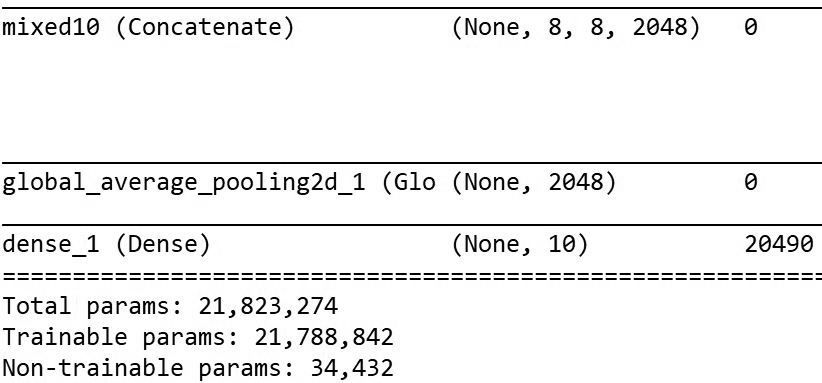
\includegraphics[scale=1]{img/3_inception-standard.jpg}
\end{adjustbox}
\end{figure}
\end{minipage}%
\begin{minipage}{.5\textwidth}
\begin{figure}[H]
\begin{adjustbox}{width=\textwidth, center}
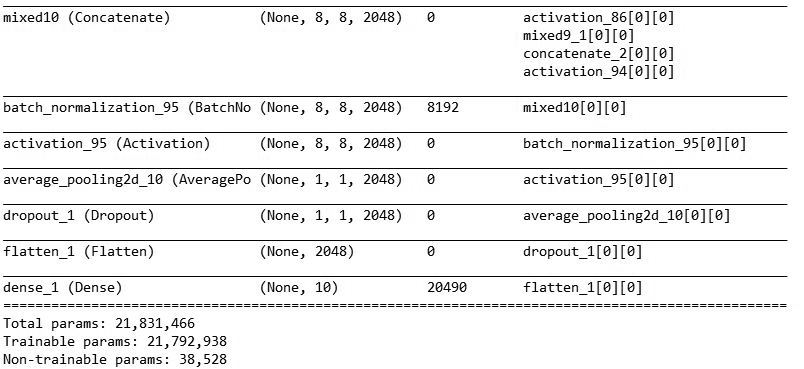
\includegraphics[scale=1]{img/3_inception-pawara.jpg}
\end{adjustbox}

\end{figure}
\end{minipage}
\caption{Standardmäßiger Aufbau des \textit{Inception V3} Netzes (links) und Änderungen an den letzten Schichten des \textit{Inception V3} Netzes von Pawara et al. \cite{pawaraWebsiteCode} (rechts).}
\label{fig:inceptionAenderungen}
\end{figure}


\subsection{Trainsize}
Um zu untersuchen, wie sich die Anzahl der zur Verfügung stehenden Trainingsdaten auf die Klassifikationsgenauigkeit der Netze auswirkt, wird für jede Kombination der anderen Parameter mit einer eingeschränkten Trainingsmenge von 10, 20, 50, 80 und 100 Prozent trainiert. Dabei werden die zur aktuellen Konfiguration der anderen Parameter gehörenden Testdaten unverändert verwendet, lediglich die Trainingsdaten werden auf eine Teilmenge eingeschränkt.\\

Im Quellcode von Pawara et al. \cite{pawaraWebsiteCode} wird bei jedem Trainingsdurchlauf eine neue Teilmenge zufällig bestimmt, was zu zufällig auftretenden Ausreißern durch gut oder schlecht gewählte Teilmengen führt.
Daher werden die Einteilungen in Teilmengen in dieser Bachelorarbeit einmalig zufällig bestimmt und für alle Trainingsdurchläufe in gleicher Form benutzt. So wird z.B. bei dem Training des \textit{ResNet-50} Netzes und einer 20-prozentigen Trainsize die gleiche Teilmenge des Datensatzes verwendet wie bei dem Training von \textit{Inception V3} mit 20 Prozent Trainsize. Die Vergleichbarkeit der Ergebnisse verschiedener Netze und der beiden Klassifikationsschemata ist daher hoch und es kommt nicht zu zufälligen Ausreißern.


\subsection{vortrainierte Gewichte}
Als weiterer Trainingsparameter wird unterschieden, ob die Netze von Grund auf, also \textit{from \textbf{Scratch}}, oder mit bereits vorab trainierten Gewichten initialisiert werden und lediglich ein \textbf{Finetuning} stattfindet. Die vorab trainierten Gewichte wurden auf dem ImageNet Datensatz \cite{imagenet} trainiert.
Dabei ist jedoch das OvA Klassifikationsschema im Vorteil, da die vorab auf ImageNet \cite{imagenet} trainierten Gewichte ebenfalls mit Hilfe eines OvA Klassifikationsschemas trainiert wurden.\\

Die initiale Learning-Rate beträgt wie bei den Experimenten von Pawara et al. \cite{pawaraPaper} für das Training \textit{from Scratch} $0.001$ und für \textit{Finetuning} $0.0001$ und wird in beiden Fällen alle 50 Epochen um einen Faktor von $0.1$ verringert. Jedoch wird im Falle von \textit{Scratch} 200 Epochen lang trainiert, bei \textit{Finetuning} lediglich 100 Epochen lang.



\section{Ausführung der Jobs auf Palma II}
\label{ch:methodik_palma}
Da durch die hohe Anzahl an verschiedenen Trainingsparametern (s. Kapitel \ref{ch:methodik_parameter}) sehr viele verschiedene Netze trainiert werden müssen, wurden für das Training die Grafikkarten (s. Tabelle \ref{tab:palmaGPUs}) des High-Performance-Computing Clusters \textit{Palma II} der Universität Münster \cite{palma2} verwendet.\\
Auf Grund von laufenden Berechnungen anderer Benutzer und technischen Ausfällen waren nicht immer alle Grafikkarten verfügbar. So standen während meinen Experimenten wegen Hardwareproblemen beispielsweise leider nur die Hälfte der insgesamt 40 RTX 2080 Grafikkarten zur Verfügung.

Außerdem konnten für die Experimente mit TensorFlow \cite{tensorflow} die Titan XP GPUs gar nicht verwendet werden, da der dort installierte Grafiktreiber nicht die erforderliche CUDA-Version unterstützt hat.

\begin{figure}[H]
\begin{tabular}{|c|c|}
\hline 
Grafikkarten-Modell & Anzahl \\ 
\hline 
NVIDIA Tesla V100-SXM2 16GB & 4 \\ 
\hline 
NVIDIA GeForce RTX 2080 Ti 11GB & bis zu 40\\
\hline
NVIDIA TITAN RTX 24GB & 4\\
\hline
NVIDIA TITAN Xp 12 GB & 8\\
\hline
\end{tabular} 
\caption{Maximale Anzahl an zur Verfügung stehenden Grafikkarten auf Palma II \cite{palma2}.}
\label{tab:palmaGPUs}
\end{figure}

Zum Training wurde für jede Kombination an Trainingsparametern (s. Kapitel \ref{ch:methodik_parameter}) ein Job mit Hilfe des Slurm Workload Managers \cite{slurm} gestartet, dem dann zum frühestmöglichen Zeitpunkt irgendeine der freien Grafikkarten zugewiesen wurde. Die zur Verfügung stehende Prozessorleistung von 6 Kernen pro Job war für alle Experimente ausreichend und stellte keinen limitierenden Faktor dar.

Lediglich der benötigte Arbeitsspeicher war für die Experimente mit TensorFlow \cite{tensorflow} und Cifar10 \cite{cifar10} so hoch, dass nur wenige Jobs gleichzeitig ausgeführt werden konnten. Dadurch entstanden sehr lange Wartezeiten bis alle Jobs abgearbeitet worden sind, weshalb die Experimente mit Cifar10 \cite{cifar10} sich auf \textit{ResNet-50 Scratch} beschränken.

